%!TEX root = draft.tex

\section{Reference Implementation}
\label{sec:reference implementation}

%In this section, we propose an abstract implementation called reference implementation, which will be used as specification in simulation proof of later section.

We present a generic definition of a CRDT reference implementations as labeled transition systems. This definition is parametrized by a specification $Spec$ defining the abstract semantics of the CRDT's operations.
%sec:specifications and consistencies

A labeled transition system (LTS, for short) is a tuple $A = (Q,\Sigma,\rightarrow,q_0)$, where $Q$ is a set of states, $\Sigma$ is an alphabet of transition labels, $\rightarrow \subseteq Q \times \Sigma \times Q$ is a transition relation and $q_0$ is the initial state. An execution of $A$ is defined as usual by a sequence of transitions starting from the initial state $q_0$. A trace is the sequence of transition labels from an execution. We say that $A$ is deterministic, if for each state $q$ and each transition label $\alpha$, $q$ has at most one $\rightarrow$ successor with transition label $\alpha$.


\begin{figure}[t]
  \centering
  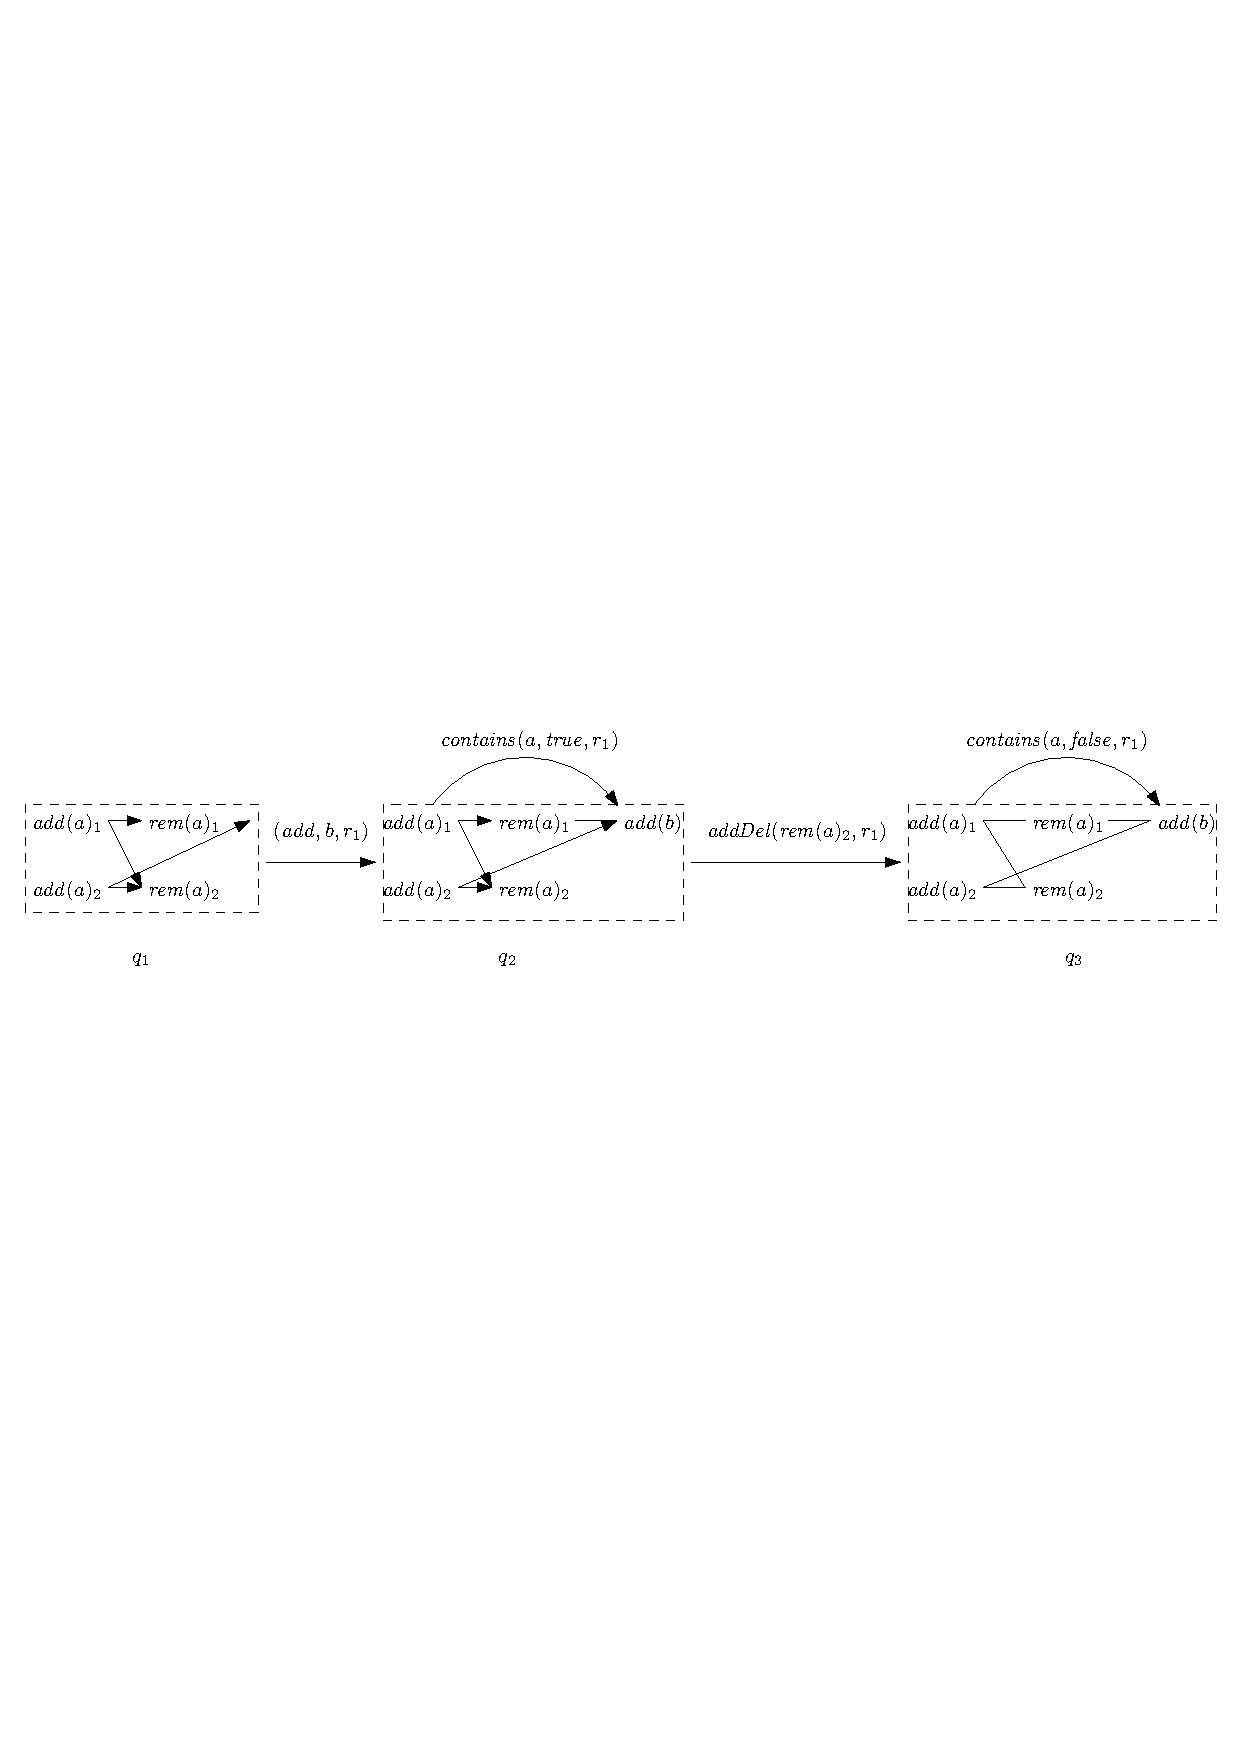
\includegraphics[width=1 \textwidth]{figures/PIC-RImp.pdf}
%\vspace{-10pt}
  \caption{Reference implementation for OR-set. Arrow of same replica represents replica order, while arrow between different replica represents delivery order.}
  \label{fig:reference implementation for OR-set}
\end{figure}

Each state of the reference implementation is a history, which for succinctness, contains only update operations, together with an arbitration order (which has the same meaning as in annotated histories) and a \emph{delivery} relation $del$ which is a ``more succinct'' substitute of the visibility relation: for two operations $o_1$ and $o_2$ submitted at replicas $r_1$ and $r_2$, respectively, $del(o_1,o_2)$ denotes the fact that $o_2$ is the first operation submitted to $r_2$ after the operation $o_1$ is delivered to $r_2$. We write $del(o_1,r_2)$ when $o_1$ is delivered after the last operation submitted to $r_2$. For instance, consider the execution fragment depicted in \figurename~\ref{fig:reference implementation for OR-set} (this is extracted from a reference implementation of the OR-set). In state $q_1$, $(add(a)_2,r_1) \in \mathit{del}$ (denoted by the edge going to the end of the replica $r_1$) means that the effect of $add(a)_2$ is delivered to replica $r_1$ after all the operations submitted at $r_1$ ($add(a)_1$ and $rem(a)_1$) happened, while $(add(a)_1,rem(a)_2) \in \mathit{del}$ means that the effect of $add(a)_1$ is delivered to replica $r_2$ at a time point earlier than when $rem(a)_2$ is submitted and later than when $add(a)_2$ is submitted. The visibility relation can be obtained as the union of $\mathit{ro}$ and the composition of $\mathit{del}$ with $\mathit{ro}$. The reference implementation has two kinds of transitions: transitions labeled by operations which may increase the history and possibly the arbitration order (query operations leave the history stored in the state unchanged) and transitions labeled by $\mathit{addDel}(\_,\_)$ which increase the delivery relation. A transition labeled by an $\ell$ operation submitted to replica $r$ is enabled when the operation context at the newest time-point of replica $r$ is in $\mathit{Spec}(\ell)$. An example of such a transition is the one from $q_1$ to $q_2$ in \figurename~\ref{fig:reference implementation for OR-set} or the self-loops in $q_2$ and $q_3$. The transition from $q_2$ to $q_3$ is an example of a transition that increases the delivery relation. Such transitions make the reference implementation deterministic.

%%We introduce a new relation $\mathit{del}$ called delivery relation to capture the intuition that CRDT only broadcast effect of one operation.
%
%%Since CRDTs normally does not use speculative execution, the annotated history increase monotonously during transitions of $\mathit{Spec}$.
%
%
%{\color {red}Let us use the example of \figurename~\ref{fig:reference implementation for OR-set} to explain how to model specification $\mathit{Spec}$ as a deterministic LTS $\mathit{RImp}(\mathit{Spec})$.
%
%\begin{itemize}
%\setlength{\itemsep}{0.5pt}
%\item[-] Each state of $\mathit{Spec}$ is an annotated history. Since CRDT normally does not use speculative execution, the annotated history increase monotonously during transitions of $\mathit{Spec}$. For simplicity these annotated history only contains update operations. We introduce a new relation $\mathit{del}$ called delivery relation to capture the intuition that CRDT only broadcast effect of one operation.
%
%
%\item[-] To do a $\ell$ operation on replica $r$, we check whether the operation context of the newest time-point of replica $r$ is in $\mathit{Spec}(\ell)$. If $\ell$ is query, then we have a loop transition, as the self-loop of $q_2$ in \figurename~\ref{fig:reference implementation for OR-set}; if $\ell$ is update, we increasing the annotated history by put a $\ell$ operation in the newest time-point of replica $r$, as the transition from $q_1$ to $q_2$ in \figurename~\ref{fig:reference implementation for OR-set}.
%
%\item[-] To make LTS be deterministic, we make the event of when a operation becomes visible to a replica also transition label. For example, the transition from $q_2$ to $q_3$ in \figurename~\ref{fig:reference implementation for OR-set} represents that $-a_2$ begins to be visible to replica $r_1$. Thus, every change to visibility relation is explicitly.
%\end{itemize} }

Formally, the reference implementation $\mathit{RImp}(\mathit{Spec}) = (Q,\Sigma,\rightarrow,q_0)$ is constructed as follows:

%\todo{Again, what is the purpose of $\mathit{li}$ and $correct$ ? The implementation should be a transition system like in the first section. No additional elements in the tuples.}

\begin{itemize}
\setlength{\itemsep}{0.5pt}
\item[-] Each state $(O,\mathit{ro},\mathit{del},\mathit{arb}) \in Q$ contains four tuples: $O$ is a set of update operations, $\mathit{ro}$ is the replica order, $\mathit{del} \subseteq (O \times O) \cup (O \times \mathbb{R})$ is the delivery relation, and $\mathit{arb}$ is the arbitration order.

%Each state of $Q$ records the set of updates already executed, when they were delivered to the different replicas, and the arbitration order.

    %Each state $(O,\mathit{ro},\mathit{del},\mathit{arb}) \in Q$ contains four tuples: $O$ is a set of update operations where each operation in $O$ has unique operation identifier; $\mathit{ro}$ is the replica order and $(O,\mathit{ro})$ a history; $\mathit{del} \subseteq (O \times O) \cup (O \times \mathbb{R})$ is a relation that records operation delivery and is called deliver order. {\color {red}Assume $o_2$ happens in replica $r_2$. $(o_1,o_2) \in \mathit{del}$ represents that the time point of delivering the effect of $o_1$ to replica $r_2$ is after all operations of replica $r_2$ that happens earlier than $o_2$, and before the time point  $o_2$ happens}. $(o,r) \in \mathit{del}$ represents that the effect of $o$ is delivered to replica $r$ after the time point of the last operation of replica $r$. we require $\mathit{del}$ to only relate operations with different replica identifier; $\mathit{arb} \subseteq O \times O$ is the arbitration order.
%\todo{$vis$ shouldn't be in the state.}

%\item[-] $\Sigma$ contains two kinds of transition labels: The first is operation labels tagged with replica identifier and arbitration order, in the form $(m,a,b,r,\mathit{arb})$, where $m \in \mathbb{M}, a,b \in \mathbb{D}, r \in \mathbb{R}$, and $arb \subseteq O \times O$; The second kind is events representing the points in time where operations are delivered, in the form $addDel(o,r)$, where $o \in \mathbb{O}, r \in \mathbb{R}$.


%\item[-] $\Sigma$ contains two kinds of transition labels: The first is operation labels tagged with replica identifier and modification of arbitration order, in the form $(m,a,b,r,ind)$, where $m \in \mathbb{M}, a,b \in \mathbb{D}, r \in \mathbb{R}$, and $ind \in \mathbb{N}$. Here $ind = 0$ means that the arbitration order does not change, while $ind >0$ means that the arbitration order is changed by inserting the newly generated operations into $ind$-th position; The second kind is events representing the points in time where operations are delivered, in the form $addDel(o,r)$, where $o \in \mathbb{O}, r \in \mathbb{R}$.

\item[-] $\Sigma$ contains two kinds of transition labels: $m(a,b,r,\mathit{arb})$ which represents the fact that an $m(a) \Rightarrow b$ operation is submitted at replica $r$ and the arbitration order is changed into $\mathit{arb}$ (the reason of using $\mathit{arb}$ in the transition label is to make $\mathit{RImp}(\mathit{Spec})$ deterministic) and $\mathit{addDel}(o,r)$ which represents the fact that operation $o$ begins to be visible to replica $r$. The transition label $m(a,b,r,\mathit{arb})$ could be simplified by giving just the index of this operation in the arbitration order instead of the full arbitration. We prefer this version to simplify the technical exposition.

%$\Sigma$ contains two kinds of transition labels: The first is operation labels tagged with replica identifier and arbitration order, in the form $(m,a,b,r,\mathit{arb})$, where $m \in \mathbb{M}, a,b \in \mathbb{D}, r \in \mathbb{R}$, and $\mathit{arb}$ is the arbitration order. The second kind is events representing the points in time where operations are delivered, in the form $addDel(o,r)$, where $o \in \mathbb{O}, r \in \mathbb{R}$.

\item[-] $\rightarrow \subseteq Q \times \Sigma \times Q$ is the transition relation. The transition rules of $\rightarrow$ can be found in \figurename~\ref{fig:transition rules of RImpSpec}, and related notions are defined as follows:


    \begin {itemize}

%    \item[-] the visibility relation $\mathit{vis}=(\mathit{del}\circ\mathit{ro})\cup\mathit{ro}$

    \item[-] $\mathit{visTo}(O,r,\mathit{del}) = \mathit{ro}|_r\cup \{ \mathit{del}^{-1}(o) \vert o \in \mathit{ro}|_r \} $ is the set of operations that are currently visible to replica $r$.
    %Here we require $\mathit{vis}$ to be acyclic and irreflexive, and $\mathit{vis}^{-1}$ to be finite.

    %Let $\mathit{vis} = \mathit{del} \cdot \mathit{ro}$ be the visibility relation. We further require $\mathit{vis}$ to be acyclic and irreflexive, and $\mathit{vis}^{-1}$ to be finite. Let $visTo(O,r,\mathit{vis}) = \{ vis^{-1}(o') \vert o'=(\_,r,\_) \in O \} \cup (vis^{-1}(r))$ be the set of operations that are visible to newest time point of replica $r$ or some operations of replica $r$.

    \item[-] %{\color {red}$f_{\mathit{ctxt}}$ is a function that generate possible operation contexts if $o$ is done. It needs to guess new arbitration relation if necessary:}
      given $q = (O,\mathit{ro},\mathit{del},\mathit{arb})$ and $o=(\_,r,\_) \notin O$, ${\mathit{ctxt}}(q,o)$ returns the potential operation context of $o$ in a state reached from $q$ by an $o$ labeled transition, i.e., a tuple $(O',\mathit{vis}',\mathit{arb}')$, where $O' = \mathit{visTo}(O,r,\mathit{del})$, $\mathit{vis}'$ is the projection of $\mathit{vis}=(\mathit{del}\circ\mathit{ro})\cup\mathit{ro}$ on $O'$, and $\mathit{arb}'$ is the projection of $\mathit{arb}$ on $O'$.

        %\begin{itemize}
        %\setlength{\itemsep}{0.5pt}
        %\item[-] $O' = visTo(O,r,\mathit{vis}) \cup \{ o \}$.

        %\item[-] $\mathit{vis'} = \mathit{vis} \uparrow_{(O' \times O')} \cup \{ (o',o) \vert (o',r) \in \mathit{vis} \}$.

        %\item[-] If $o$ is an update operation, then $\mathit{arb}'$ is obtained from $\mathit{arb} \uparrow_{(O' \times O')}$ by possibly adding relations between $O'$ and $\{ o \}$; Else, $\mathit{arb}' = \mathit{arb} \uparrow_{(O' \times O')}$.
        %\item[-] $\mathit{arb}'$ is obtained from $\mathit{arb} \uparrow_{(O' \times O')}$ by possibly insert update operation $o$ into some place.
        %\end{itemize}

    %\item[-] $f_{\mathit{ar}}(\mathit{arb},o)$ returns an arbitration order that is obtained from $\mathit{arb}$ by possibly adding relations between $O$ and $\{ o \}$.
%    \item[-] {\color {red}$\mathit{rand}(\mathit{arb},o)$ randomly returns an arbitration order that is obtained from $\mathit{arb}$ by either do nothing or insert update $o$ into some place.}

    \item[-] $\mathit{ro} \oplus o = ro \cup \{ (o',o) \vert o' = (\_,r,\_) \in O \}$ and $\mathit{del} \oplus o$ returns a new delivery relation obtained from $del$ by transforming each $(o',r)$ into $(o',o)$.

    \item[-] $\mathit{arb}\oplus o$ denotes all the arbitration orders obtained by inserting $o$ in the total order represented by $\mathit{arb}$.

    %\item[-] $pos(l,a)$ returns the position of $a$ in list $l$.
    \end{itemize}
Note that, for simplicity, query operations don't modify the arbitration order.
%    {\color {red}Note that the arbitration order may be changed only when new operation happens, while delivery does not change arbitration order.}

\item[-] $q_0=(\emptyset,\emptyset,\emptyset,\emptyset)$ is the initial state.
\end{itemize}

\begin{figure}[ht]
Transitions increasing the delivery relation:
\[
\begin{array}{l c}
\bigfrac{ o \in O\quad (o,r)\notin visTo(O,r,\mathit{del}) }
{ (O,\mathit{ro},\mathit{del},\mathit{arb}) {\xrightarrow{addDel(o,r)}} (O,\mathit{ro},\mathit{del} \cup \{ (o,r) \},\mathit{arb}) } %{\mathit{Delivery}}
\end{array}
\]


%\[
%\begin{array}{l c}
%\bigfrac{ o=(\ell,r,\_) \notin O, \exists x, x \in f_{\mathit{ctxt}}((O,\mathit{ro},\mathit{del},\mathit{arb}),o) \wedge x \in Spec(\ell) }
%{ (O,\mathit{ro},\mathit{del},\mathit{arb}) {\xrightarrow{m(a,b,r,\mathit{arb})}} (O,\mathit{ro},\mathit{del},\mathit{arb}) } {\mathit{Query}}
%\end{array}
%\]
Transitions for submitting query operations:
\[
\begin{array}{l c}
\bigfrac{ m \in \mathbb{Q}\quad \ell = m(a) \Rightarrow b\quad o=(\ell,r,\_) \notin O\quad {\mathit{ctxt}}((O,\mathit{ro},\mathit{del},\mathit{arb}),o) \in Spec(\ell) }
{ (O,\mathit{ro},\mathit{del},\mathit{arb}) {\xrightarrow{m(a,b,r,\emptyset)}} (O,\mathit{ro},\mathit{del},\mathit{arb}) } %{\mathit{Query}}
\end{array}
\]


%\[
%\begin{array}{l c}
%\bigfrac{ o = (\ell,r,\_) \notin O, \exists x, x = (O',\_,f_{\mathit{ar}}(\mathit{arb},o) \uparrow_{O'} ) \in f_{\mathit{ctxt}}((O,\mathit{ro},\mathit{del},\mathit{arb}),o) \wedge x \in %Spec(\ell) }
%{ (O,\mathit{ro},\mathit{del},\mathit{arb}) {\xrightarrow{m(a,b,r,f_{\mathit{ar}}(\mathit{arb},o))}} (O \cup \{ o \},\mathit{ro} \oplus o ,\mathit{del} \oplus %o,f_{\mathit{ar}}(\mathit{arb},o)) } {\mathit{Update}}
%\end{array}
%\]
Transitions for submitting updates:
\[
\begin{array}{l c}
\bigfrac{ 
\begin{array}{c}
 m \in \mathbb{U}\quad \ell = m(a) \Rightarrow b\\
o = (\ell,r,\_) \notin O\quad \mathit{arb}'\in \{\mathit{arb}\}\cup \mathit{arb}\oplus o
\quad
  {\mathit{ctxt}}((O,\mathit{ro},\mathit{del},\mathit{arb}'),o) \in Spec(\ell) 
\end{array}
  }
{ (O,\mathit{ro},\mathit{del},\mathit{arb}) {\xrightarrow{m(a,b,r,\mathit{arb}')}} (O \cup \{ o \},\mathit{ro} \oplus o ,\mathit{del} \oplus o,\mathit{arb}') } %{\mathit{Update}}
\end{array}
\]

\caption{Transition rules of $\rightarrow$}
\label{fig:transition rules of RImpSpec}
\end{figure}

%\FloatBarrier
The reference implementation corresponding to the OR-set specification in Example~\ref{} is obtained as an instantiation of the above definition where even for update operations ($\mathit{add}$ and $\mathit{rem}$) the arbitration order contained in transition labels is $\emptyset$. Similarly, for the list specification in Example~\ref{}, only the transition labels corresponding to $\mathit{add}$ operations contain a non-empty arbitration order.

%
%
%
%\begin{itemize}
%\setlength{\itemsep}{0.5pt}
%\item[-] {\color {red}For OR-set, $f_{\mathit{ctxt}}$ and $\mathit{rand}(\mathit{arb},o)$ uses only arbitration order $\emptyset$.}
%
%\item[-] For distributed list: In $f_{\mathit{ctxt}}$, $\mathit{arb}'$ is obtained from $\mathit{arb} \uparrow_{O'}$ by inserting $o$ into some place if $o$ is a $add$ operation, or unchanged otherwise. $\mathit{rand}(\mathit{arb},o)$ returns an arbitration order that is obtained from $\mathit{arb}$ by insert $o$ into some place if $o$ is a $add$ operation, or unchanged otherwise.
%\end{itemize}

Assuming deterministic specifications $\mathit{Spec}$ and that the operation identifier generation is deterministic, the reference implementation $\mathit{RImp}(\mathit{Spec})$ is itself deterministic.
The annotated history $(O,\mathit{ro},\mathit{vis},\mathit{arb})$ corresponding to an execution $q_0 {\xrightarrow{\alpha_1}} q_1 \ldots$ of $\mathit{RImp}(\mathit{Spec})$ can be defined as expected: $O$ is the set of operations included in transition labels, $\mathit{vis}$ is defined from replica order and the delivery relation, and $\mathit{arb}$ is the union of the arbitration orders included in each $q_i$. A history $(O,\mathit{ro})$ can be extracted from an execution in a similar way. Let $\mathit{his}(\mathit{RImp}(\mathit{Spec}))$ be the set of histories corresponding to executions of $\mathit{RImp}(\mathit{Spec})$. The following result shows that any (annotated) history generated by $\mathit{RImp}(\mathit{Spec})$ satisfies CRVC (see Appendix \ref{sec:appendix definitions and proofs of section reference implementation}).

\begin{theorem}
\label{theorem:histories of reference implementation are SRV consistent}
For each $h \in \mathit{his}(\mathit{RImp}(\mathit{Spec}))$, $h$ is CRVC w.r.t $\mathit{Spec}$.
\end{theorem}

\noindent
{\bf Causal delivery.} The reference implementations defined above can be constrained so that operation delivery is consistent with the causal order between operations.
Given a state $q = (O,\mathit{ro},\mathit{del},\mathit{arb})$, an operation $o_1\in O$ \emph{happens-before} an operation $o_2\in O$, denoted by $o_1 <_{\mathit{hb}} o_2$, if $(o_1,o_2) \in (\mathit{ro}\cup \mathit{del})^*$. A state of the reference implementation satisfies \emph{causal delivery} if for each pair of update operations $(o_1,o_2)$ in this state such that $o_1 <_{\mathit{hb}} o_2$, $o_2$ is delivered to replica $r$ only when $o_1$ has already been delivered to replica $r$. For example, the state $q_3$ in \figurename~\ref{fig:reference implementation for OR-set} satisfies causal delivery, e.g., $add(a)_2 <_{\mathit{hb}} rem(a)_2$ and $add(a)_2$ has already been delivered to replica $r_1$ when $rem(a)_2$ is delivered to $r_1$.

To abstract CRDT implementations that assume causal delivery of messages (which can be defined as for operations), we use a class of reference implementations $\mathit{RImp}(\mathit{Spec})_{\mathit{cd}}$ where operations are delivered in the causal order. Formally, this consists in strengthening the transition rule corresponding to delivery events as follows:

%The reference implementation with causal delivery of $Spec$ is given as an LTS $RImp(Spec)_{\mathit{cd}} = (Q,\Sigma,q_0,\rightarrow)$. $RImp_{\mathit{cd}}(Spec)$ can be obtained from $RImp(Spec)$ by only changing the transition rules of delivery into the following:

\medskip
%\setlength{\itemsep}{0.5pt}
$\begin{array}{l c} \bigfrac{o \in O\quad o\mbox{ is minimal w.r.t $<_{\mathit{hb}}$ in }\{ o' \vert o' \in O \wedge o' \notin \mathit{visTo}(O,r,\mathit{del}) \}} {(O,\mathit{ro},\mathit{del},\mathit{arb}) {\xrightarrow{addDel(o,r)}} (O,\mathit{ro},\mathit{del} \cup \{ (o,r) \},\mathit{arb})} \end{array}$

%The following lemma states that $RImp(Spec)_{\mathit{cd}}$ contains all the traces of $RImp(Spec)$ that are causal delivery. Its proof can be found in Appendix \ref{sec:appendix definitions and proofs of section reference implementation}.

%\begin{lemma}
%\label{lemma:RImpcdSpec contains all the sequences of RImpSpec that are causal delivery}
%$\llbracket RImp(Spec)_{\mathit{cd}} \rrbracket = \{ t \vert t \in \llbracket RImp(Spec) \rrbracket \wedge t$ satisfies causal delivery $\}$.
%\end{lemma}




\forget{
\noindent {\bf Example 3. $RImp(S_{\mathit{ORS}})$}: function $ctxt$ and predicate $cor$ are defined as follows:
\begin{itemize}
\setlength{\itemsep}{0.5pt}
\item[-] Given $o=(\_,r,\_)$ and $q=(O,ro,del,\emptyset)$, $ctxt(q,o) = (visTo(O,r,vis),<_1,\emptyset)$, where $<_1 = vis \uparrow_{(O_1 \times O_1)} - \{ (o_1,o_2) \vert o_2 \notin Minus(q,o_1), \exists o_3, o_1 {\xrightarrow{vis}} o_3 {\xrightarrow{vis}} o_2, o_1,o_2 \in visTo(O,r,vis), o_3 \notin visTo(O,r,vis) \}$.

Here $Minus(q,o_1)$ is defined as follows: (1) if $lab(o_1)=add(a)$, then $Minus(q,o_1) = \{o_2 \vert lab(o_2)=rem(a), o_1 {\xrightarrow{vis}} o_2, \neg \exists o_3, ( lab(o_3) = rem(a) ) \wedge ( o_1 {\xrightarrow{vis}} o_3 {\xrightarrow{vis}} o_2 ) \}$, (2) otherwise, $Minus(q,o_1) = \emptyset$.

\item[-] $cor((O,ro,del,arb))$ holds, if

    \begin{itemize}
    \setlength{\itemsep}{0.5pt}
    \item[-] $arb= \emptyset$.

    \item[-] $\forall o \in O$, if $lab(o)=rem(a)$, then $\exists o', o \in Minus(q,o')$.
    \end{itemize}
\end{itemize}

\noindent {\bf Example 4. $RImp(S_{\mathit{list}})$}: function $ctxt$ and predicate $cor$ are defined as follows:

\begin{itemize}
\setlength{\itemsep}{0.5pt}
\item[-] Given $q = (O,ro,del,arb)$ and $o =(\_,r,\_)$, $ctxt(q,o) = ( O_1 ,<_1, arb_1 )$, where $O_1 = visTo(O,r,vis)$, $<_1 = vis \uparrow_{(O_1 \times O_1)}$, and $arb_1$ is as follows: (1) if $lab(o)=add(\_)$, then $arb_1$ is a total order generated by adding $o$ into some place of $arb$, (2) otherwise, $arb_1 = arb$. We also require that

\item[-] $cor((O,ro,del,arb))$ holds, if

    \begin{itemize}
    \setlength{\itemsep}{0.5pt}
    \item[-] $arb$ is a acyclic and irreflexive total order over $add$ operations of $O$.

    \item[-] For each operation $o \in O$, $f(o) \neq \mathit{Undef}$.
    \end{itemize}
\end{itemize}
}


















%%% Local Variables:
%%% mode: latex
%%% TeX-master: "draft"
%%% End:
